\documentclass[14pt]{article}

\usepackage{fancyhdr}
\usepackage{extramarks}
\usepackage{amsmath}
\usepackage{amsthm}
\usepackage{amsfonts}
\usepackage{amssymb}
\usepackage{tikz}
\usepackage[plain]{algorithm}
\usepackage{algpseudocode}
\usepackage{enumitem}
\usepackage{relsize}
\usepackage{scrextend}
\usepackage{graphicx}

\usetikzlibrary{automata,positioning}

%
% Basic Document Settings
%

\topmargin=-0.45in
\evensidemargin=0in
\oddsidemargin=0in
\textwidth=6.5in
\textheight=9.0in
\headsep=0.25in

\linespread{1.1}

\pagestyle{fancy}
\lhead{\hmwkAuthorName}
\chead{\hmwkClass\ (\hmwkClassInstructor): \hmwkTitle}
\rhead{\firstxmark}
\lfoot{\lastxmark}
\cfoot{\thepage}

\renewcommand\headrulewidth{0.4pt}
\renewcommand\footrulewidth{0.4pt}

\setlength\parindent{0pt}

%
% Create Problem Sections
%

\newcommand{\enterProblemHeader}[1]{
    \nobreak\extramarks{}{Problem \arabic{#1} continued on next page\ldots}\nobreak{}
    \nobreak\extramarks{Problem \arabic{#1} (continued)}{Problem \arabic{#1} continued on next page\ldots}\nobreak{}
}

\newcommand{\exitProblemHeader}[1]{
    \nobreak\extramarks{Problem \arabic{#1} (continued)}{Problem \arabic{#1} continued on next page\ldots}\nobreak{}
    \stepcounter{#1}
    \nobreak\extramarks{Problem \arabic{#1}}{}\nobreak{}
}

\setcounter{secnumdepth}{0}
\newcounter{partCounter}
\newcounter{homeworkProblemCounter}
\setcounter{homeworkProblemCounter}{1}
\nobreak\extramarks{Problem \arabic{homeworkProblemCounter}}{}\nobreak{}

%
% Homework Problem Environment
%
% This environment takes an optional argument. When given, it will adjust the
% problem counter. This is useful for when the problems given for your
% assignment aren't sequential. See the last 3 problems of this template for an
% example.
%
\newenvironment{homeworkProblem}[1][-1]{
    \ifnum#1>0
        \setcounter{homeworkProblemCounter}{#1}
    \fi
    \section{Problem \arabic{homeworkProblemCounter}}
    \setcounter{partCounter}{1}
    \enterProblemHeader{homeworkProblemCounter}
}{
    \exitProblemHeader{homeworkProblemCounter}
}

%
% Homework Details
%   - Title
%   - Due date
%   - Class
%   - Section/Time
%   - Instructor
%   - Author
%


\newcommand{\hmwkClass}{CS 219}
\newcommand{\hmwkTitle}{Homework\ \#5}
\newcommand{\hmwkDueDate}{October 5th, 2016}
\newcommand{\hmwkDueTime}{4:00pm}
\newcommand{\hmwkClassInstructor}{Dr. Egbert}
\newcommand{\hmwkAuthorName}{Matthew J. Berger}

%
% Title Page
%

\title{
    \vspace{2in}
    \textmd{\textbf{\hmwkClass:\ \hmwkTitle}}\\
    \normalsize\vspace{0.1in}\small{Due\ on\ \hmwkDueDate\ at \hmwkDueTime}\\
    \vspace{0.1in}\large{\textit{\hmwkClassInstructor}}
    \vspace{3in}
}

\author{\textbf{\hmwkAuthorName}}
\date{}

\renewcommand{\part}[1]{\textbf{\large Part \Alph{partCounter}}\stepcounter{partCounter}\\}

%
% Various Helper Commands
%

% Useful for algorithms
\newcommand{\alg}[1]{\textsc{\bfseries \footnotesize #1}}

% Alias for the Solution section header
\newcommand{\solution}{\textbf{\large Solution:}}

% Alias for answers
\newcommand{\answer}{\textbf{\large Answer: }}

\begin{document}

\maketitle

\pagebreak

\begin{homeworkProblem}
	\textbf{Review Questions}
	\begin{itemize}
		\item[1.1.)] What general categories of functions are specified by computer instructions?\\
		\answer
		The categories are processor I/O, processor memory, data processing, and c control.
		\item[1.2.)] List and briefly define the possible states that define an instruction execution?\\
		\answer
		\begin{itemize}
			\item \textbf{IAC - Instruction Address Calculation} - Determine the address of the next instruction to be executed
			\item \textbf{IF - Instruction Fetch} - Read instruction from its memory location into the processor.
			\item \textbf{OAC - Operand Address Calculation} - If the operation references an operand stored in memory or one that is available via I/O, then determine its address.
			\item \textbf{OF - Operand Fetch} - Fetch the operand from memory or read it in from I/O.
			\item \textbf{Data Operation} - Perform the operation indicated in the instruction.
			\item \textbf{OS - Operand Store} - Write the result into memory or out to I/O.
		\end{itemize}
		\item[1.3.)] List and briefly define two approaches to dealing with multiple interrupts?\\
		\answer
		\begin{itemize}
			\item \textbf{ISR - Interrupt Service Routines} - Priorities are assigned to each different type of interrupt. ISR's with higher priorities can interrupt lower priority ISR's, resulting in the lower priority ISR being put on the stack until that ISR is completed.
			\item \textbf{Disabling Interrupts} - The processor can ignore specific interrupts and those will remain pending, only to be checked after the processor has enabled interrupts.
		\end{itemize}
		\item[1.4.)] What types of transfers must a computer's interconnection structure (e.g., bus) support?\\
		\answer
		\begin{itemize}
			\item Memory to processor and processor to memory
			\item I/O to processor and processor to I/O
			\item I/O to memory and memory to I/O
		\end{itemize}
		\item[1.5.)] List and briefly define the QPI protocol layers.\\
		\answer
		\begin{itemize}
			\item \textbf{Physical} - Wires that carry signals, circuitry, logic for other features required for transmitting and receiving binary data.
			\item \textbf{Link} - Responsible for flow control and reliable transmission.
			\item \textbf{Routing} Allows for direction of packets.
			\item \textbf{Protocol} - The high-level set of rules for exchanging packets of data between devices.
		\end{itemize}
		\item[1.6.)] List and briefly define the PCIe protocol layers.\\
		\answer
		\begin{itemize}
			\item \textbf{Physical} - Wires that carry signals, circuitry, logic for other features required for transmitting and receiving binary data.
			\item \textbf{Link} - Responsible for flow control and reliable transmission.
			\item \textbf{Transmission} - Generates and consumes data packets that are then used to implement load/store data transfer systems. Also handles flow control of the packets between various components on a link.
		\end{itemize}
	\end{itemize}
\end{homeworkProblem}

\pagebreak

\begin{homeworkProblem}

	\begin{itemize}
		\item[2.1)] The hypothetical machine of Figure 3.4 in the book also has two I/O instructions:
	\begin{itemize}
		\item 0011 = load AC from I/O
		\item 0111 = store AC to I/O
	\end{itemize}
	
	In these cases, the 12-bit address identifies a particular I/O device. Show the program execution (using the format of Figure 3.5) for the following program:
	\begin{enumerate}
		\item Load AC from device 5
		\item Add contents of memory location 940.
		\item Store AC to device 6.
	\end{enumerate}
	Assume that the next value retrieved from device 5 is 3 and that location 940 contains a value of 2.\\
	\answer
	\begin{itemize}
		\begin{table}[h]
		\def\arraystretch{1.5}%
		\item \hfil
			\begin{tabular}{|c|c|}
				\hline
				Address & Memory \\
				\hline
				300 & 3 0 0 5 \\
				\hline
				301 & 5 9 4 0 \\
				\hline
				302 & 7 0 0 6 \\
				\hline
				... & ... \\
				\hline
				940 & 0 0 0 2 \\
				\hline
			\end{tabular}
		\end{table}
	\end{itemize}
	The memory contains 300: 3005, 301: 5940, and 302:7006. This means the program instructions will have to do the following steps:
	\begin{enumerate}
		\item \(3005 \rightarrow IR\)
		\item \(3 \rightarrow AC\)
		\item \(5940 \rightarrow IR\)
		\item \(3 + 2 = 5 \rightarrow AC\)
		\item \(7006 \rightarrow IR\)
		\item \(AC \rightarrow Device\ 6\)
	\end{enumerate}
	\pagebreak
	\item[2.2)] A combinational circuit is used to control a seven-segment display or decimal digits, as shown in Figure 11.35 in the book. The circuit has four inputs, which provide the four-bit code used in packed decimal representation $(0_10=000,\ ...\ , 9_10=10001)$. The seven outputs define which segments will be activated to display a given decimal digit. Note that some combinations of inputs and outputs are not needed.
		\begin{itemize}
			\item[a.)] Develop a truth table for this circuit.
			\item[b.)] Express the truth table in SOP form.
			\item[c.)] Express the truth table in POS Form.
		\end{itemize}
		\answer
		
		N/A
	\item[2.3)] Implement the full adder of Figure 11.20 with just five gates. (Hint: Some of the gates are XOR gates.)\\
	\answer
	From wikipedia:
	
	\centerline{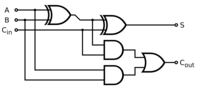
\includegraphics{fa.png}}
	\item[2.4)] Consider Figure 11.20 from the book. Assume that each gate produces a delay of 10 ns. Thus, the sum output is valid after 20 ns and the carry output after 20 ns. What is the total add time for a 32-bit adder
		\begin{itemize}
			\item[a.)] Implemented without carry lookahead, as in Figure 11.19 in the book.
			\item[b.)] Implemented with carry lookahead using 8-bit adders, as in Figure 11.21 from the book.
		\end{itemize}
		
		\answer
		
		N/A
	\end{itemize}
\end{homeworkProblem}

\end{document}
